%==============================================================
%  Figura 5.3 - Stima del rischio e riduzione del rischio
%  Adattamento in italiano della Figura 5.3 dell'IFA Report 2/2017
%  Disegno vettoriale: coordinate in cm, origine sulla scala del rischio
%==============================================================
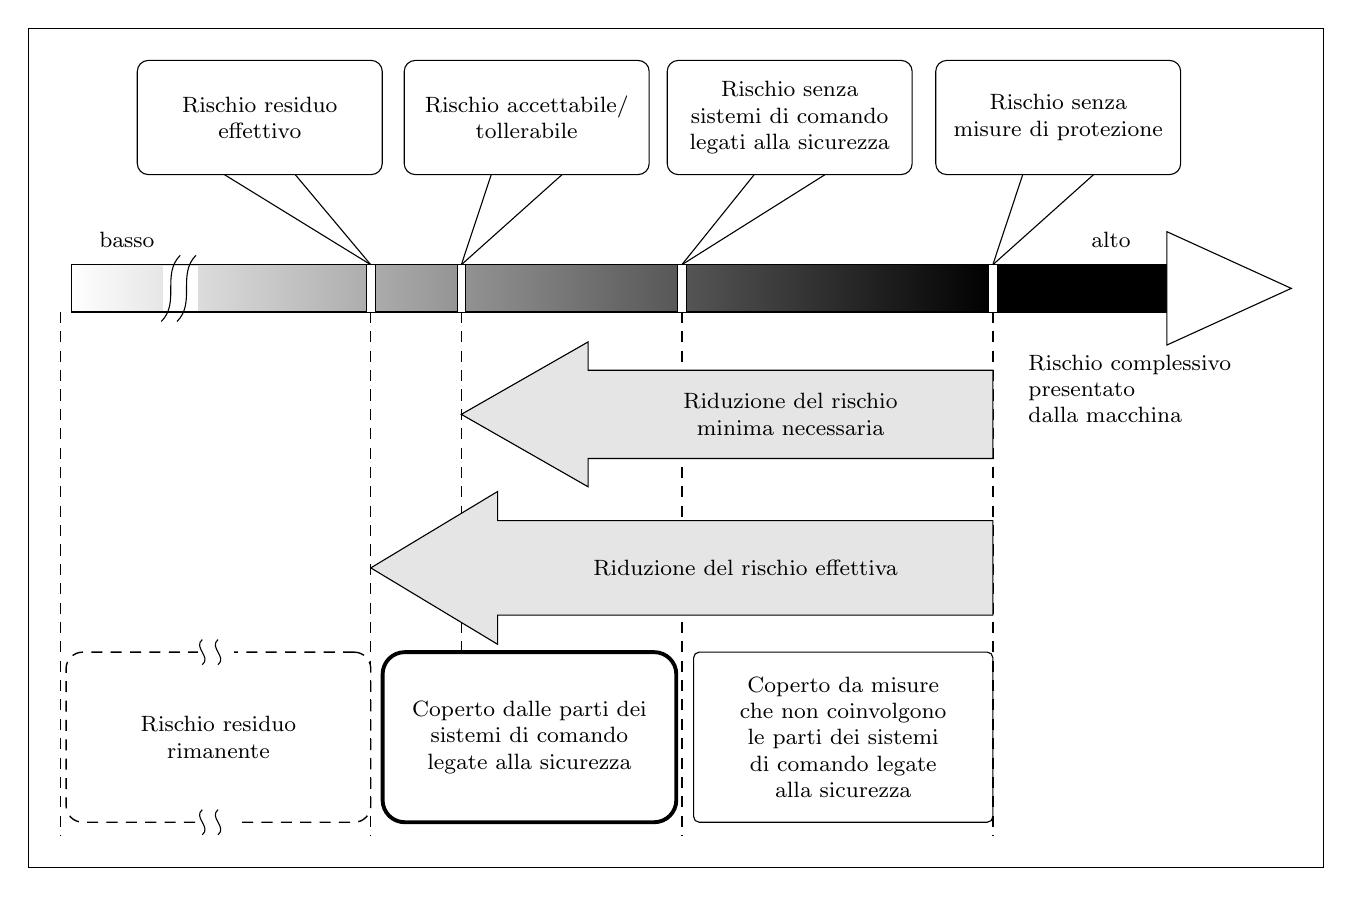
\begin{tikzpicture}[
  font=\footnotesize,
  fdline/.style={draw=black, line width=0.4pt},
  fdbox/.style={draw=black, fill=white, line width=0.4pt, align=center, inner sep=3pt},
  fdcall/.style={fdbox, rounded corners=4pt, text width=2.9cm, minimum height=1.45cm},
  fddash/.style={draw=black, line width=0.5pt, dash pattern=on 4pt off 3pt},
  lab/.style={font=\footnotesize, inner sep=1pt}
]

%--------------------------------------------------------------
% Scala del rischio (barra sfumata con punta a freccia)
%--------------------------------------------------------------
\shade[left color=white, right color=black] (0.64,-0.30) rectangle (12.34,0.30);
\fill[black] (12.34,-0.30) rectangle (14.55,0.30);
\draw[fdline] (0.64,-0.30) rectangle (14.55,0.30);
\filldraw[fill=white, draw=black, line width=0.4pt]
  (14.55,0.30) -- (14.55,0.72) -- (16.13,0) -- (14.55,-0.72) -- (14.55,-0.30) -- cycle;

% interruzione della scala
\fill[white] (1.80,-0.29) rectangle (2.24,0.29);
\draw[fdline] (1.78,-0.42) .. controls (2.02,-0.18) and (1.78,0.18) .. (2.02,0.42);
\draw[fdline] (1.98,-0.42) .. controls (2.22,-0.18) and (1.98,0.18) .. (2.22,0.42);

% tacche bianche in corrispondenza dei quattro livelli di rischio
\foreach \x in {4.44, 5.59, 8.39, 12.34}{
  \filldraw[fill=white, draw=black, line width=0.3pt] (\x-0.055,-0.30) rectangle (\x+0.055,0.30);
}

\node[lab, anchor=west] at (0.95,0.62) {basso};
\node[lab, anchor=west] at (13.55,0.62) {alto};

%--------------------------------------------------------------
% Fumetti dei quattro livelli di rischio
%--------------------------------------------------------------
\node[fdcall] (c1) at (3.03,2.17) {Rischio residuo\\ effettivo};
\node[fdcall] (c2) at (6.42,2.17) {Rischio accettabile/\\ tollerabile};
\node[fdcall] (c3) at (9.76,2.17) {Rischio senza\\ sistemi di comando\\ legati alla sicurezza};
\node[fdcall] (c4) at (13.17,2.17) {Rischio senza\\ misure di protezione};

\foreach \cx/\px in {3.03/4.44, 6.42/5.59, 9.76/8.39, 13.17/12.34}{
  \draw[fdline] (\cx-0.45,1.445) -- (\px,0.30);
  \draw[fdline] (\cx+0.45,1.445) -- (\px,0.30);
}

%--------------------------------------------------------------
% Linee tratteggiate di riferimento
%--------------------------------------------------------------
\foreach \x in {0.50, 4.44, 8.39, 12.34}{ \draw[fddash] (\x,-0.30) -- (\x,-6.95); }
\draw[fddash] (5.59,-0.30) -- (5.59,-4.62);

%--------------------------------------------------------------
% Frecce di riduzione del rischio
%--------------------------------------------------------------
\filldraw[fill=black!10, draw=black, line width=0.4pt]
  (12.34,-1.04) -- (7.20,-1.04) -- (7.20,-0.68) -- (5.59,-1.60)
  -- (7.20,-2.52) -- (7.20,-2.16) -- (12.34,-2.16) -- cycle;
\node[align=center, text width=5.0cm] at (9.77,-1.60)
  {Riduzione del rischio\\ minima necessaria};

\filldraw[fill=black!10, draw=black, line width=0.4pt]
  (12.34,-2.95) -- (6.05,-2.95) -- (6.05,-2.58) -- (4.44,-3.55)
  -- (6.05,-4.52) -- (6.05,-4.15) -- (12.34,-4.15) -- cycle;
\node[align=center, text width=5.6cm] at (9.20,-3.55)
  {Riduzione del rischio effettiva};

\node[lab, anchor=north west, align=left, text width=3.3cm] at (12.75,-0.80)
  {Rischio complessivo\\ presentato\\ dalla macchina};

%--------------------------------------------------------------
% Riquadri inferiori: ripartizione del rischio
%--------------------------------------------------------------
\node[draw=black, line width=0.5pt, dash pattern=on 4pt off 3pt, rounded corners=6pt,
      align=center, text width=3.4cm, minimum width=3.87cm, minimum height=2.16cm]
      (bA) at (2.505,-5.70) {Rischio residuo\\ rimanente};

\node[draw=black, line width=1.4pt, rounded corners=8pt,
      align=center, text width=3.3cm, minimum width=3.73cm, minimum height=2.16cm]
      (bB) at (6.455,-5.70) {Coperto dalle parti dei\\ sistemi di comando\\ legate alla sicurezza};

\node[draw=black, line width=0.4pt, rounded corners=2pt,
      align=center, text width=3.5cm, minimum width=3.80cm, minimum height=2.16cm]
      (bC) at (10.44,-5.70) {Coperto da misure\\ che non coinvolgono\\ le parti dei sistemi\\ di comando legate\\ alla sicurezza};

% interruzione del riquadro del rischio residuo
\foreach \y in {-4.62, -6.78}{
  \fill[white] (2.24,\y-0.06) rectangle (2.70,\y+0.06);
  \draw[fdline] (2.30,\y-0.16) .. controls (2.42,\y-0.06) and (2.18,\y+0.06) .. (2.30,\y+0.16);
  \draw[fdline] (2.50,\y-0.16) .. controls (2.62,\y-0.06) and (2.38,\y+0.06) .. (2.50,\y+0.16);
}

%--------------------------------------------------------------
% Cornice
%--------------------------------------------------------------
\draw[draw=black, line width=0.5pt]
  ([shift={(-0.40,0.40)}]current bounding box.north west) rectangle
  ([shift={(0.40,-0.40)}]current bounding box.south east);

\end{tikzpicture}
